\subsection{Umsetzung der Anwendung}
\label{technische-umsetzung-umsetzung-der-anwendung}
Dieser Abschnitt erläutert den Aufbau der Szenen in Unity, um einen Überblick der erforderlichen Komponenten zu erhalten. Zunächst wird darauf eingegengen, wie eine Szene in AR Foundation aufgebaut ist. Dann wird ein Überblick über die verwendeten Skripte und deren Funktion in der Anwendung geschaffen, damit sich interessierte Entwickler schnell zurecht finden. 

Im Anschluss wird die Anbindung mit der REST-API erklärt. Die Antwort der API und die damit erzeugten Effekte werden aufgezeigt.

\subsubsection{Grundaufbau der AR Szenen in Unity}
\label{technische-umsetzung-platzierung-auf-einer-beliebigen-flaeche}
% Was wird gebraucht?
% Szenenaufbau
Bei der Erstellung eines neuen Projekts in Unity kann ein Standard Template für die Entwicklung von AR ausgewählt werden. Dieses beinhaltet Beispielszenen, Assets und die benötigten Packages. Diese können in normalen Unity Projekten im Package Manager installiert werden. Die benötigten Packages sind wie in Abbildung \ref*{fig:anwendung-umsetzung-packages} zu sehen in einem Gesamtpaket für AR vorhanden.

\begin{figure}[H]
    \centering
    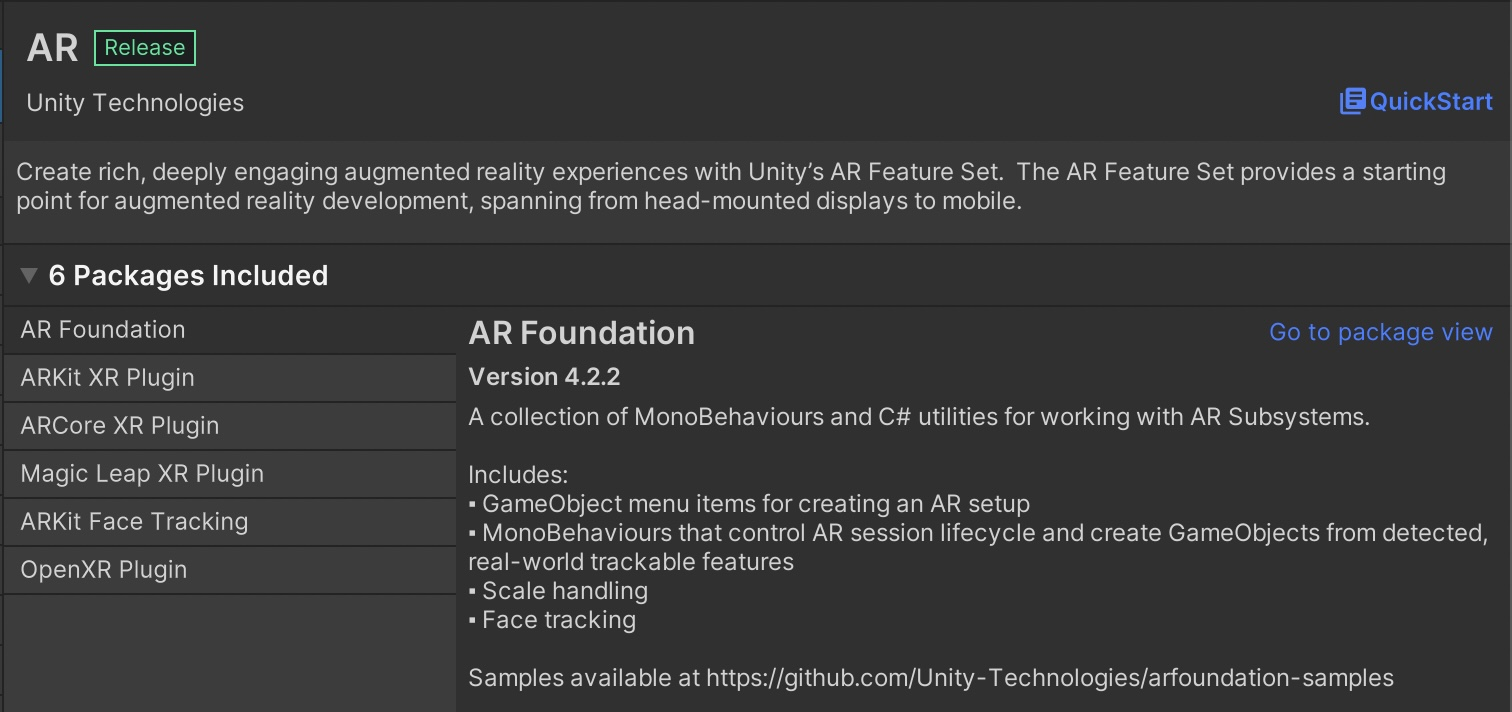
\includegraphics[width=8cm]{img/anwendung/technisch/ar-setup/setup-ar-unity.jpg}
    \caption{Die benötigten Packages im Package Manager.}
    \label{fig:anwendung-umsetzung-packages}
\end{figure}

Damit ARCore Zugriff auf die Packages hat, muss in den Projekteinstellungen unter \textit{XR Plug-in Management} Einstellungen vorgenommen werden. Unter dem Tab für Android muss ARCore als Plug-in Provider aktiviert werden. Damit wird das Plug-In für ARCore aktiviert und es kann auf die Kamera des Smartphones zurückgegriffen werden.

Eine einfache AR Szene besteht aus drei wichtigen Szenenobjekten, die in Abbildung \ref*{fig:anwendung-umsetzung-szenenaufbau} zu sehen sind: die \textit{AR Session}, die \textit{AR Session Origin} und die \textit{AR Camera}.

\begin{figure}[H]
    \centering
    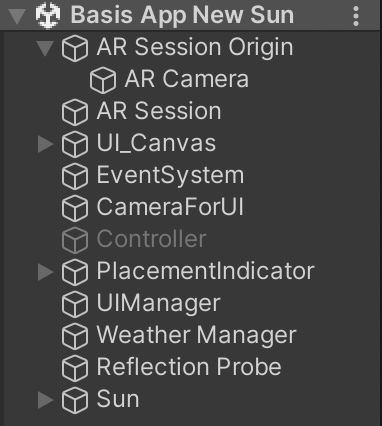
\includegraphics[width=5cm]{img/anwendung/technisch/ar-setup/setup-szenenaufbau.jpg}
    \caption{Der Szenenaufbau für die Position auf beliebigen Flächen.}
    \label{fig:anwendung-umsetzung-szenenaufbau}
\end{figure}

Die \textit{AR Session} ist ein \textit{GameObject}, dass das AR Session Skript enthält. Dieses sorgt für das Tracking. Wird das AR Session Skript deaktiviert, werden keine Schlüsselpunkte mehr erzeugt. Wird das Skript wieder aktivert, wird versucht die bestehenden Schlüsselpunkte weiterhin zu nutzen.

\begin{figure}[H]
    \centering
    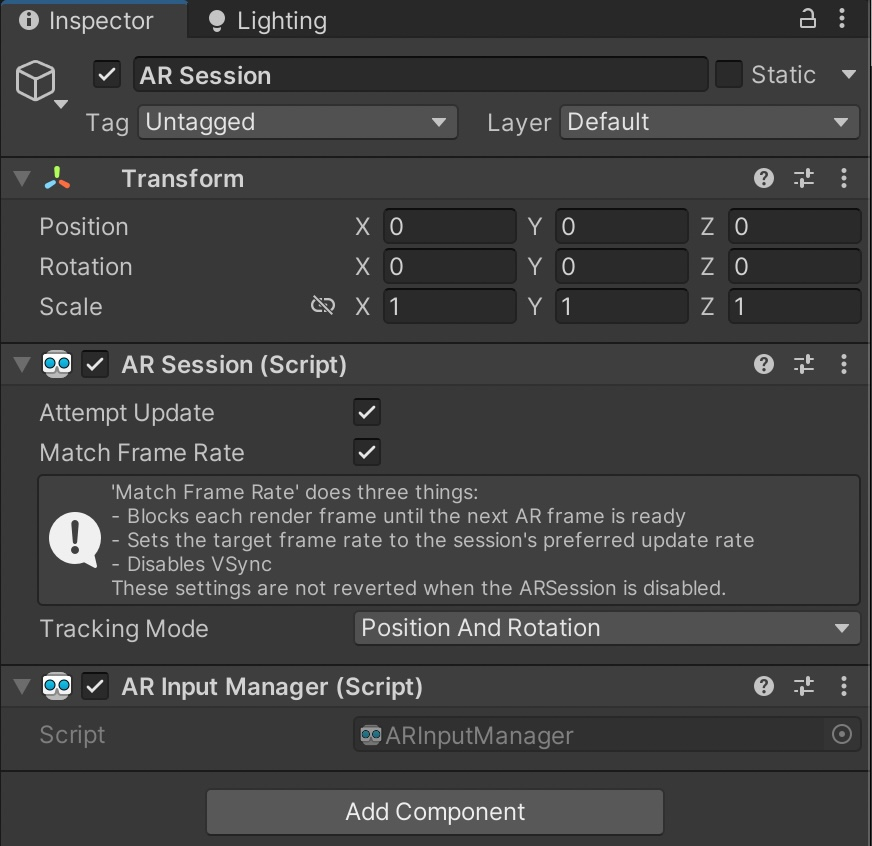
\includegraphics[width=6cm]{img/anwendung/technisch/ar-setup/setup-arsession.jpg}
    \caption{Die AR Session.}
    \label{fig:anwendung-umsetzung-arsession}
\end{figure}

Die \textit{AR Session Origin} ist auch ein \textit{GameObject}, an dem das AR Session Origin Skript hängt. Es transformiert die Trackable Objekte, wie z.B.  Schlüsselpunkte und Flächen, in ihre finale Position, Orientierung und Skalierung in das Weltkoordinatensystem von Unity. Die Skalierung der AR Session Origin bestimmt damit auch die Skalierung der Objekte in der Szene. Ist die Skalierung auf 0.1 gesetzt, so werden die Objekte in der Szene um den Faktor 0.1 verkleinert. Dies ist ein wichtiger Aspekt für die korrekte Skalierung der Gebäude, damit diese in der GPS Platzierung in der korrekten Größe dargestellt werden. Außerdem werden an der AR Session Origin die Skripte angehängt, die für einige ARCore Funktionen zuständig sind. So hängt für diese Anwendung der AR Plane Manager und der AR Raycast Manger daran.

\begin{figure}[H]
    \centering
    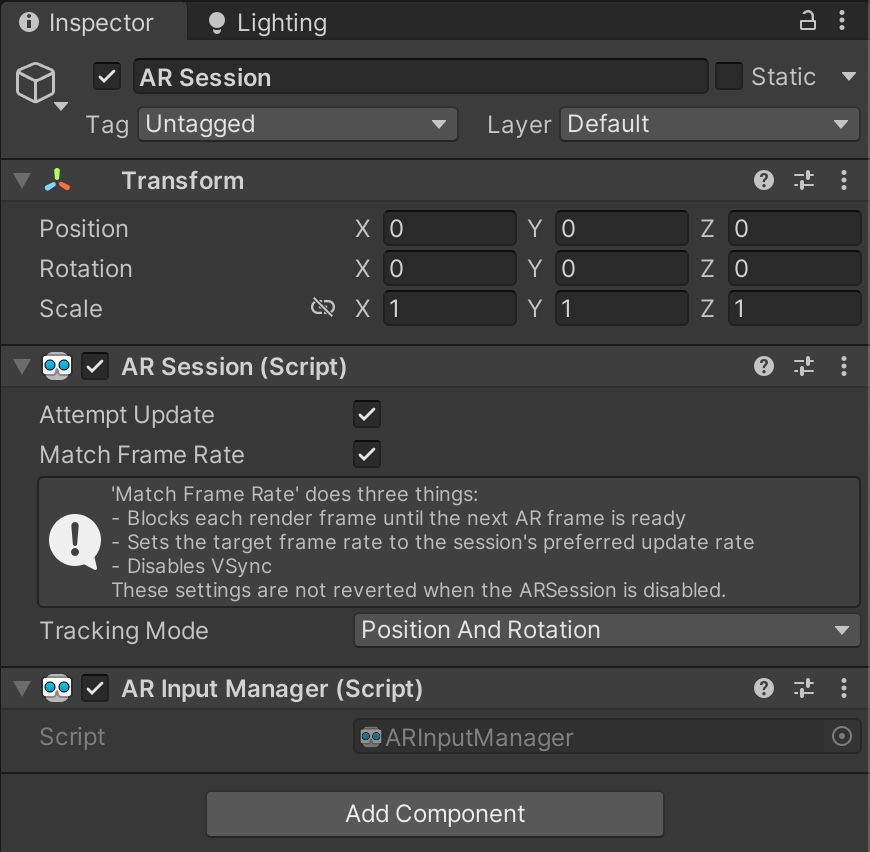
\includegraphics[width=6cm]{img/anwendung/technisch/ar-setup/setup-arsessionorigin.jpg}
    \caption{Die AR Session Origin mit dem AR Plane Manager und dem AR Raycast Manager.}
    \label{fig:anwendung-umsetzung-arsessionorigin}
\end{figure}

Das dritte Szenenobjekt ist die \textit{AR Camera}. Dies ist die Kamera von Unity mit zusätzlichen Komponenten. Diese sind der \textit{AR Camera Manager}, der \textit{AR Camera Background} und der \textit{Tracked Pose Driver}. Im AR Camera Manager wird die Light estimation und dessen Modus aktiviert. Die \textit{Facing Direction} bestimmt, ob die Front- oder die Rückkamera des Smartphones genutzt wird. Das AR Camera Background Skript sorgt dafür, dass das Kamerabild des Smartphone als Hintergrund angezeigt wird. Im Tracked Pose Driver werden Einstellungen vorgenommen, die für die Bestimmung der Position und Orientierung benötigt werden. Im Falle von AR im Smartphone wird hier festgelegt, dass die Pose über die Kamera berechnet wird. Die AR Camera wird als Kindelement der AR Session Origin eingefügt.

\begin{figure}[H]
    \centering
    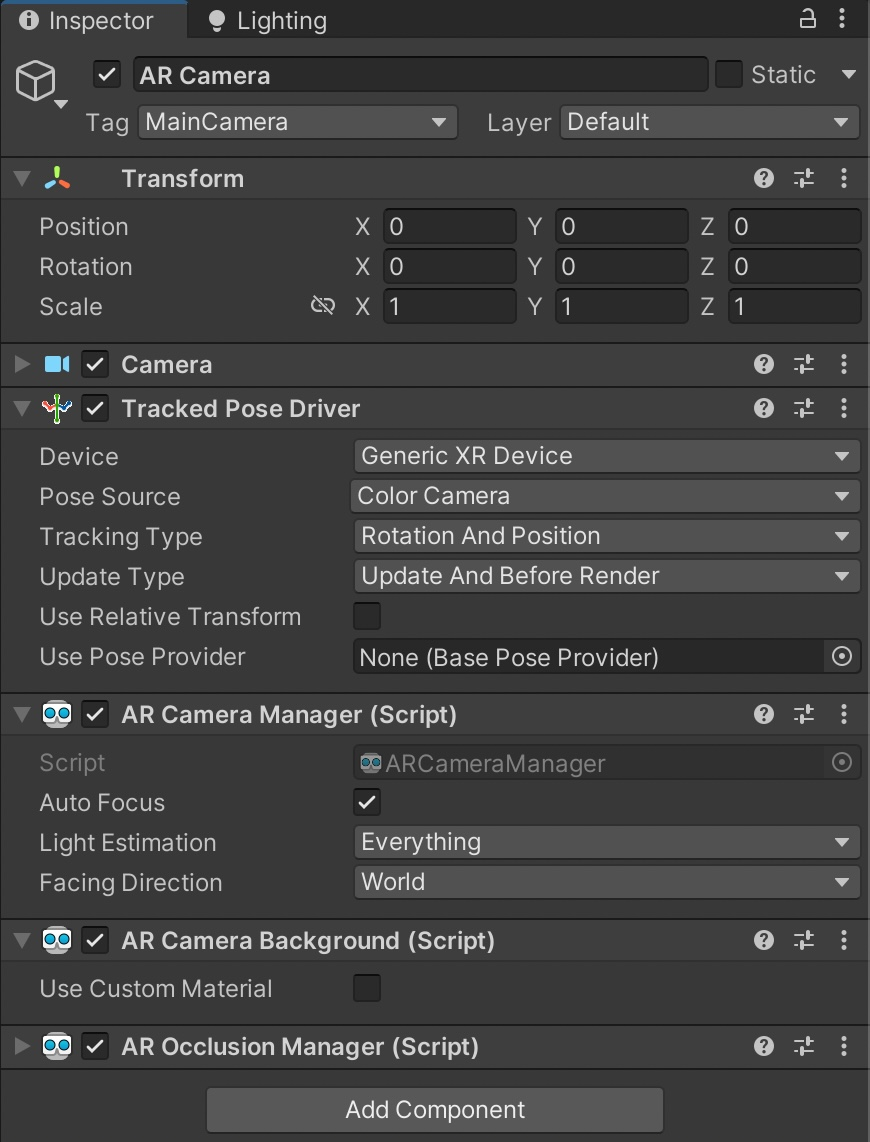
\includegraphics[width=6cm]{img/anwendung/technisch/ar-setup/setup-arcamera.jpg}
    \caption{Die AR Camera. Der Occlusion Manager aus der Depth API wird hier als Komponente eingefügt.}
    \label{fig:anwendung-umsetzung-arcamera}
\end{figure}

Diese drei Elemente werden für jede AR Anwendung in AR Foundation benötigt. Ausführliche Erklärungen zu den einzelnen Komponenten sind in der AR Foundation Dokumentation zu finden \cite*{UnityARFoundation}.

\subsubsection{Controller}
\label{technische-umsetzung-platzierung-auf-einer-beliebigen-flaeche-controller}
Der \textit{Controller} in der Szene aus Abbildung \ref*{fig:anwendung-umsetzung-szenenaufbau} ist ein \textit{GameObject}, das die Logik der Interaktionen beinhaltet. Alle Interaktionsmöglichkeiten (bis auf das User Interface) werden über dieses \textit{GameObject} geregelt. In den folgenden Abschnitt werden diese Funktionen kurz erläutert, damit ein Überblick über die verwendeten Skripte geschaffen wird.

\subsubsubsection{Platzieren auf einer beliebigen Fläche}
\label{technische-umsetzung-platzierung-normal}
Für die Platzierung der Gebäude ist das Skript \texttt{ARPlaceObjectAndMove.cs} zuständig. Wie in Kapitel \ref*{technische-umsetzung-arcore-user-interaction} erwähnt, wird in dieser Anwendung Raycast verwendet, um bei einem Hit einen Pfeil auf einer erkannten Ebene zu zeigen. Dieser dient als Placement Indicator. Wird eine Fläche erkannt, wird mit einem Tip auf dem Bildschirm das Gebäude platziert. Die Position und Orientierung wird vom letzten registrierten Hit bestimmt. Die Implementierung ist mit dem Code von Kris Schultz erfolgt\footnote{https://github.com/TheUnityWorkbench/tuw-arfoundation-demo/blob/master/Assets/Demo/ARTapToPlaceObject.cs, zuletzt aufgerufen am 13.08.2022}. Die Abbildung \ref*{fig:anwendung-umsetzung-platzierung} zeigt den Placemet Indicator und wie die das Gebäude platziert wird.

\begin{figure}[H]
    \centering
    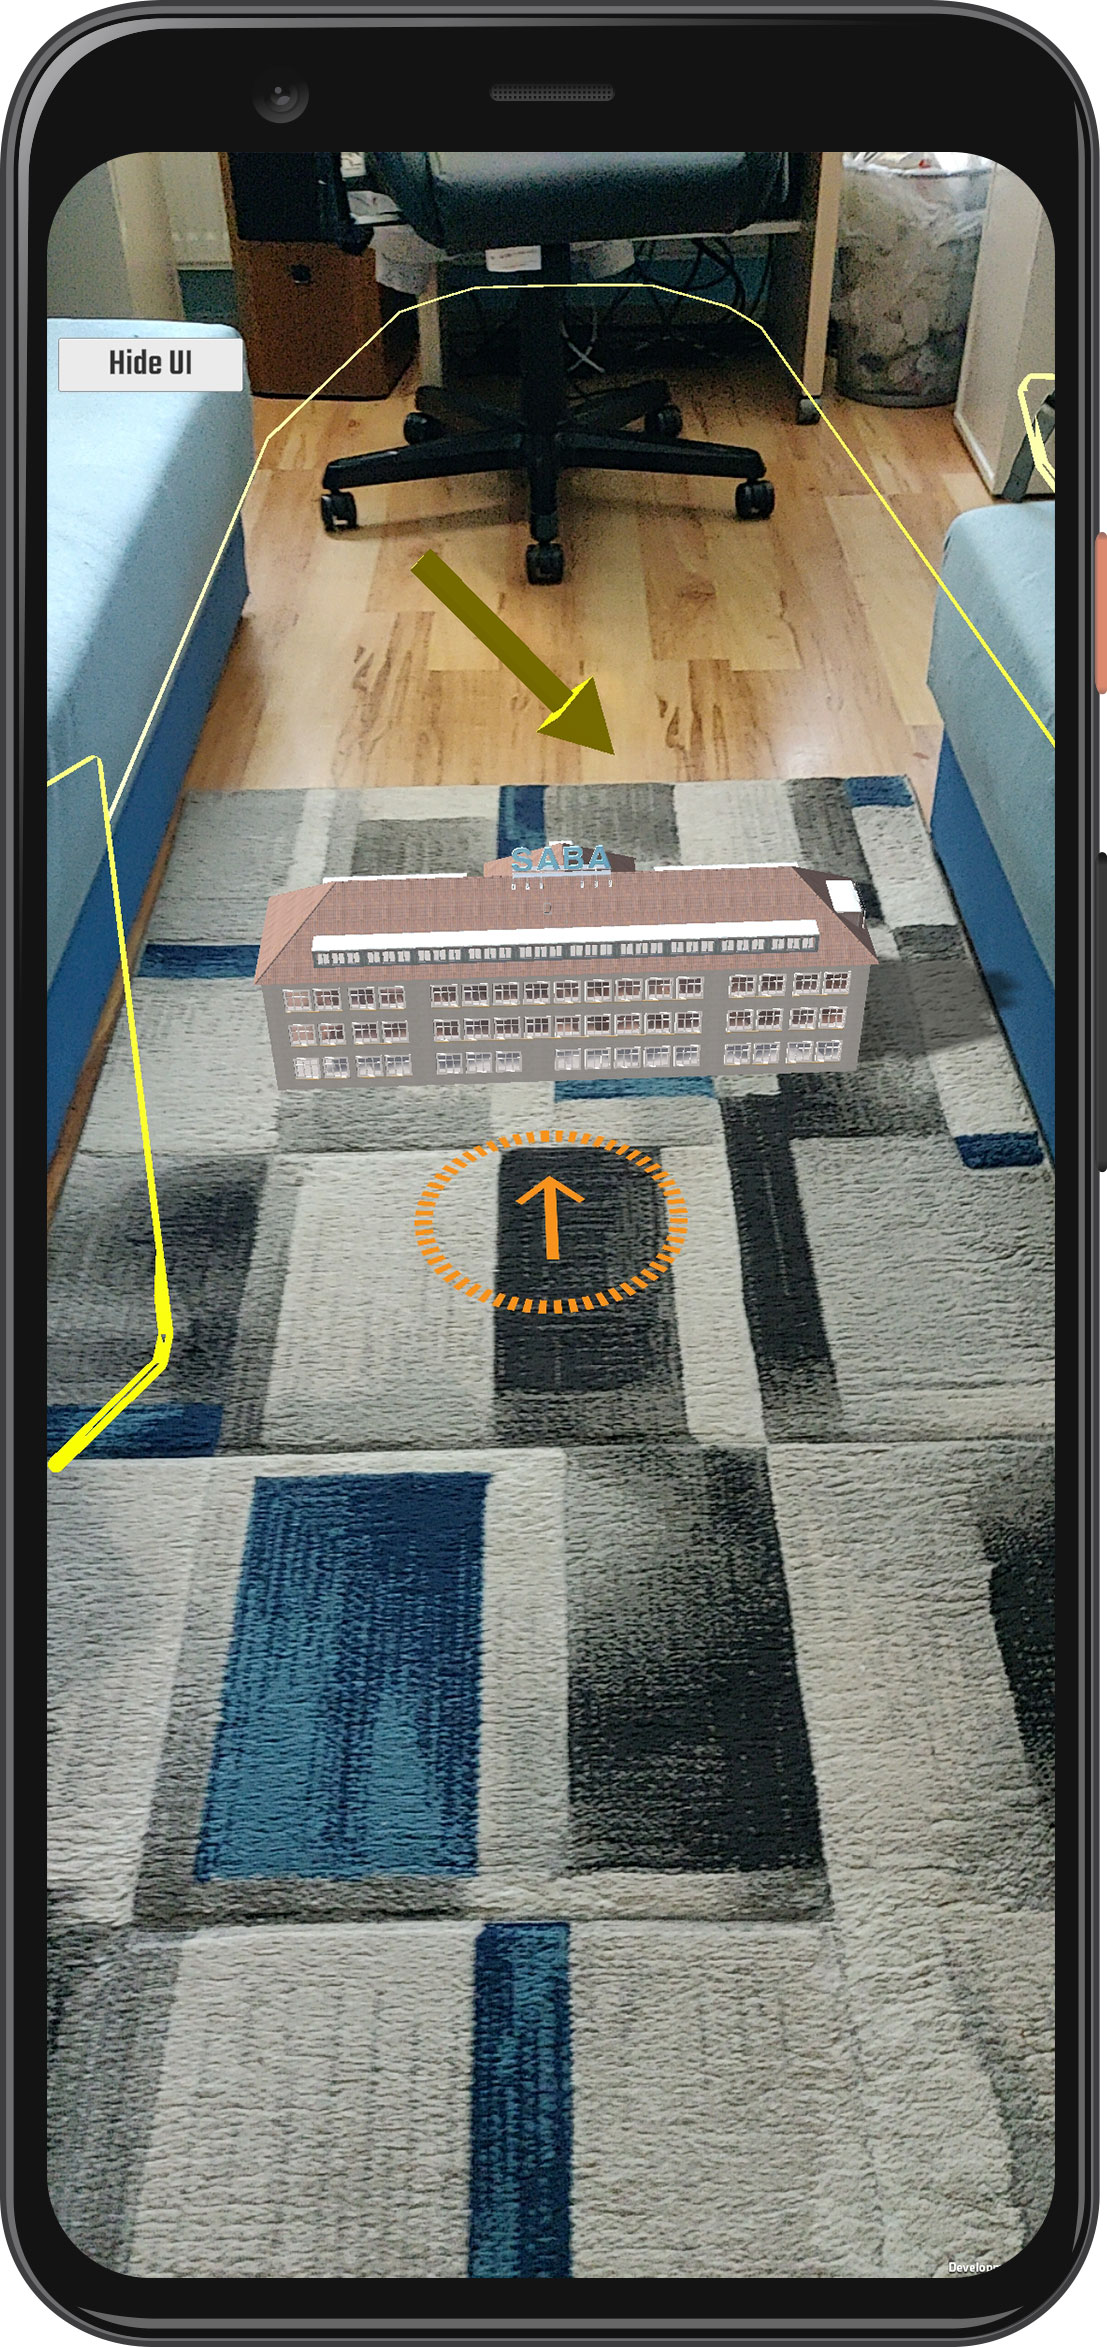
\includegraphics[width=6cm]{img/anwendung/technisch/controller/placement-indicator-beispiel.jpg}
    \caption{Der Pfeil auf dem Boden signalisiert, dass auf dieser Fläche Objekte platziert werden können.}
    \label{fig:anwendung-umsetzung-platzierung}
\end{figure}

Die Funktion \texttt{ARPlaceObject()}\footnote{unter Schultz als \texttt{PlaceObject()} benannt} wird für diese Anwendung modifiziert. Dies ist nötig, um die Funktion zu implementieren, dass das vom Nutzer ausgewählte Objekt platziert wird. Außerdem wird überprüft, ob es bereits eine Instanz des Gebäudes in der Szene gibt. Es soll nicht möglich sein ein Gebäude mehrmals zu platzieren.

Hierfür werden die aus Kapitel \ref*{konzept-der-anwendung} erwähnten BuildingGPS Scriptable Objects benötigt. Es werden zwei Listen geführt. Die Liste in Zeile 11 im unteren Code beinhaltet nur die Prefabs, die für die \texttt{Instantiate()} Funktion gebraucht wird. Die zweite Liste in Zeile 19 wird geführt, um das Scriptable Object des ausgwählten Gebäudes zu speichern. Tippt der Nutzer nach der Platzierung nochmal auf den Bildschirm, wird die ID des ausgewählten mit den ID's aus der Liste verglichen. Stimmt eine ID überein, ist das ausgewählte Gebäude bereits in der Szene vorhanden. Die \texttt{ARPlaceObject()} Funktion wird nicht ausgeführt.

\begin{lstlisting}[language=C,caption={Die \texttt{ARPlaceObject()} Funktion.},captionpos=b,label=lst:arplaceobject-funktion]
public void ARPlaceObject()
{
    //Get the selected Object from the ObjectSelection Script. This Script is attached to the UIManager.
    choosedObject = selectionMenuScript.selectedObject;
    foreach (var currentBuilding in buildings)
    {
        //Check if there is an instance of the choosed building in the scene.
        if (currentBuilding.id == choosedObject.id)
        {
            //Add the object to a list.
            listOfSpawnedObjects.Add(
                Instantiate(
                    currentBuilding.prefab,
                    placementPose.position,
                    placementPose.rotation
                )
            );
            //add the object to the building info list, in order to check earlier, if the building already exists
            listOfSpawnedObjectsBuildingInfo.Add(choosedObject);
        }
    }
} // end function ARPlaceObject()
\end{lstlisting}

\paragraph*{Pinch Funktion zur Skalierung}
Neben der Platzierung der Gebäude wird im \texttt{ARPlaceObjectAndMove.cs} Skript ermöglicht, die Gebäude zu Skalieren und auf einer Fläche zu bewegen. Die Skalierung wird dann ausgeführt, wenn zwei Finger gleichzeitg den Bildschirm berühren. Die Distanz der beiden Finger während der Pinch Bewegung bilden den Wert für die Skalierung\footnote{Der verwendete Code: https://www.youtube.com/watch?v=ISBIu6Jzfk8, zuletzt aufgerufen am 13.08.2022}.

\paragraph*{Gebäudewahl und Positionsveränderung auf einer Fläche}
Die Bewegung auf einer Fläche wird mit einem Raycast implementiert. Dabei wird ein Strahl von der Position des Touches erzeugt. Das Gebäude wird an die Position verschoben, bei der der Strahl die Fläche geschnitten hat. Der verwendete Code ist aus dem Github Repository von Dilmer Valecillos\footnote{https://github.com/dilmerv/UnityARFoundationEssentials/blob/master/Assets/Scripts/PlacementWithDraggingDroppingController.cs, zuletzt aufgerufen am 13.08.2022}.

\subsubsubsection{Objekte auswählen}
Für das auswählen der Objekte im \texttt{SelectObject()} Skript wird wieder ein Raycast genutzt. Von der Position der Mitte des Bildschirms wird ein Strahl geschickt. Wird ein Hit registriert, so wird zunächst überprüft, ob das Objekt ein Gebäude ist. Zur Identifikation werden \textit{Tags} genutzt. Unity bietet die Möglichkeit jedem GameObject einen Tag zu geben. Ein Tag ist ein String, dass als Referenz für das GameObject genutzt werden kann\footnote{https://docs.unity3d.com/Manual/Tags.html, zuletzt aufgerufen am 15.08.2022}. Wie in Abbildung \ref*{fig:anwendung-umsetzung-tags} zu sehen, bietet Unity vorgefertigte Tags. Es können auch eigene Tags definiert werden, wie in diesem Anwendungsfall der \textit{Selectable} Tag. Wird ein Gebäude identifiziert, erhält das Gebäude einen Outline Shader. Dieser fügt dem Gebäude eine Umrandung hinzu, die dem Nutzer signalisiert, dass das Gebäude ausgewählt werden kann. Mit den Button \textit{Select} und \textit{Deselect} kann der Nutzer die Gebäude auswählen und anschließend verschieben, rotieren, skalieren und entfernen.

\begin{figure}[H]
    \centering
    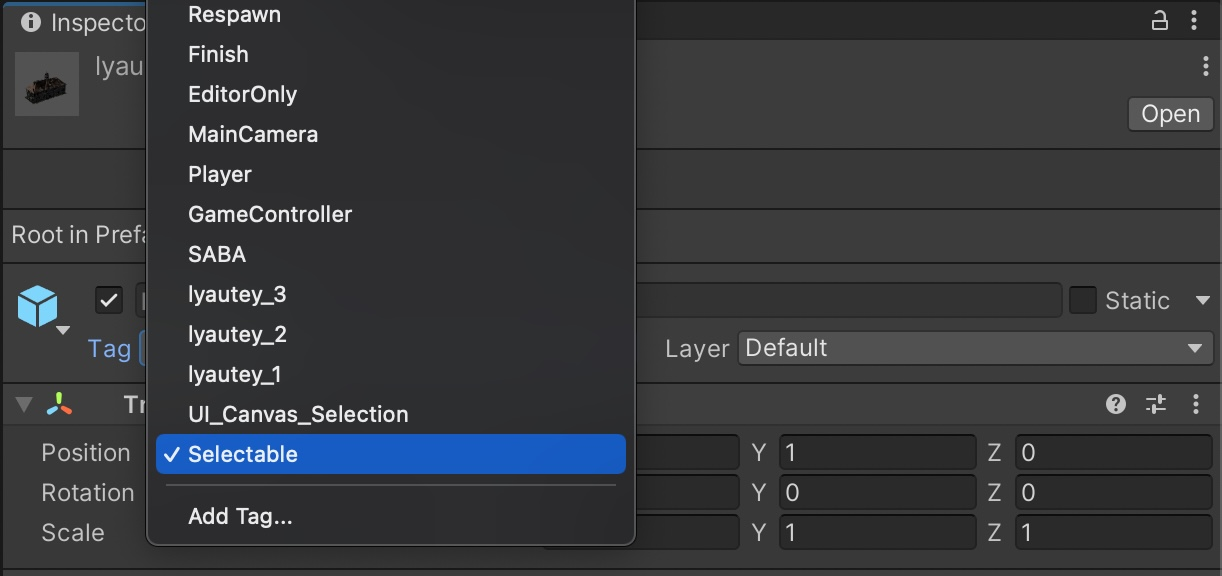
\includegraphics[width=8cm]{img/anwendung/technisch/controller/umsetzung-tags.jpg}
    \caption{Die Tag-Auswahl im Unity Inspector.}
    \label{fig:anwendung-umsetzung-tags}
\end{figure}

\paragraph*{Gebäude entfernen}
Zur Entfernung der Gebäude ist das Skript \texttt{DestroyObject.cs} zuständig. Mit dem Löschen Button wird die Funktion gestartet. Damit der Nutzer nicht aus versehen Gebäude löscht, wird ein Gebäude erst dann entfernt, wenn der Button für zwei Sekunden gedrückt wird. Es werden die zwei Listen aus dem \texttt{ARPlaceObjectAndMove.cs} Skript bearbeitet. Mit dem Befehl \texttt{Remove()} wird das jeweilige Gebäude aus den Listen entfernt und die Instanz des Gebäudes wird mit \texttt{Destroy()} zerstört.

\subsubsection{GPS Platzierung}
% Nativ nicht von AR Foundation. ARLocation aus dem Asset store
% Szenenaufbau, was wird gebraucht?
% UI
\label{technische-umsetzung-platzierung-gps}
Die Platzierung von Objekten über die GPS Informationen des Smartphones und der Angabe von GPS Längen- und Breitengraden ist nativ nicht mit AR Foundation möglich. Es können zwar GPS Informationen des Smartphones mit dem \textit{LocationService}\footnote{https://docs.unity3d.com/ScriptReference/LocationService.html, zuletzt aufgerufen am 15.08.2022} von Unity abgerufen werden. Das Platzieren von Objekten über GPS Koordinaten muss selbst implementiert werden. Hierfür wird das Asset \textit{AR + GPS Location} aus dem Asset Store benutzt\footnote{https://assetstore.unity.com/packages/tools/integration/ar-gps-location-134882, zuletzt aufgerufen am 15.08.2022}. Dieses Asset hat eine umfangreiche Dokumentation\footnote{https://docs.unity-ar-gps-location.com/, zuletzt aufgerufen am 15.08.2022}. Für das Asset werden weitere GameObjects in der Szene benötigt. In der \textit{AR Session Origin} wird ein \textit{AR Location Root} Objekt erzeugt. Außerdem wird in die Szene ein \textit{GPS Stage Object} gebraucht, das das \texttt{PlaceAtLocation.cs} Skript trägt. Dieses Objekt dient als Parent für jedes Objekt, das in der Szene platziert werden soll. Die jeweiligen GPS Koordinaten können im Inspector eingetragen werden. 

Da der Nutzer keine Auswahl hat, welches Gebäude platziert wird, wird jedes Gebäude aus der hinterlegten Datenbank platziert. Voraussetzung ist, dass das Gebäude innerhalb der eingestellten Render Distanz von Unity liegt. Ansonsten wird das in Kapitel \ref*{grp-geometrieverarbeitung-clipping} eingeführte Clipping durchgeführt und die Gebäude außerhalb des Einheitswürfels werden abgeschnitten. In dieser Anwendung ist die Render Distanz auf 250 Unity Einheiten gesetzt, was 250 Metern entspricht\footnote{https://docs.unity3d.com/ScriptReference/Camera-farClipPlane.html, zuletzt aufgerufen am 15.08.2022}. Dies genügt, um drei Gebäude nebeneinader zu platzieren. So ist es vor Ort mit den Gebäuden 2, 3 und 4 der Fall ist. 

Für die GPS Platzierung wird das \texttt{ARPlaceObjectAndMove} Skript angepasst. Die \texttt{MoveObject()} Funktion wird nicht mehr benötigt. Der untere Code zeigt die Anpassungen an der \texttt{ARPlaceObject()} Funktion. Für jedes Gebäude wird zunächst eine \texttt{Location} erzeugt. Dies ist ein Scriptable Object vom Asset\footnote{https://docs.unity-ar-gps-location.com/guide/\#locationdata, zuletzt aufgerufen am 15.08.2022}. Hier werden die Längen-, Breiten- und Höhengrade eingetragen. Diese Angaben stammen aus der Datenbank der Gebäude. Der \texttt{AltitudeMode} bestimmt, ob der eingegebene Höhengrad verwendet werden soll, oder ob eine detektierte Fläche von ARCore für die Platzierung genutzt werden soll. Da die Höhengrade in der Regel nicht sehr genau sind, werden die erkannten Flächen von ARCore genutzt. Anschließend werden Optionen gesetzt, die für die Platzierung im nächsten Schritt benötigt werden. Mit der Funktion \texttt{CreatePlacedInstance()}, die vom Asset bereitgestellt wird, wird das jeweilige Gebäude platziert.

\begin{lstlisting}[language=C,caption={Die angepasste \texttt{ARPlaceObject()} Funktion für die Platzierung mit GPS.},captionpos=b,label=lst:GPS-arplaceobject-funktion]
void ARPlaceObject()
{
    foreach (var currentBuilding in buildings)
    {
        //set new location data
        var location = new Location()
        {
            Latitude = currentBuilding.latitude,
            Longitude = currentBuilding.longitude,
            Altitude = currentBuilding.altitude,
            AltitudeMode = AltitudeMode.GroundRelative
        };
        //set options
        var options = new PlaceAtLocation.PlaceAtOptions()
        {
            HideObjectUntilItIsPlaced = true,
            MaxNumberOfLocationUpdates = 2,
            MovementSmoothing = 0.1f,
            UseMovingAverage = false
        };
        //create Instance
        spawnedObject = PlaceAtLocation.CreatePlacedInstance(
            currentBuilding.prefab,
            location,
            options,
            false
        );
        //set Rotation to fit real facing direction
        spawnedObject.transform.rotation = Quaternion.Euler(0, 0, 0);
        var currentHeading = locationProvider.CurrentHeading.heading;
        spawnedObject.transform.Rotate(
            0,
            (float)currentHeading - currentBuilding.realWorldOrientation,
            0,
            Space.World
        );
        listOfSpawnedObjects.Add(spawnedObject);
    }
}
\end{lstlisting}

\subsubsubsection{Ausrichtung der Szene nach Norden}
\label{umsetzung-gps-ausrichtung-nach-norden}
% Orientierung nach Norden
Wie in Kapitel \ref*{tracking-koordinatensysteme} erwähnt, wird beim Start einer Unity Szene die Richtung bestimmt, in die die z-Achse des Weltkoordinatensystems zeigen wird. In AR Foundation ist dies die Richtung, in die die Kamera des Smartphones zeigt. Damit die Gebäude in die richtige Richtung zeigen, müsste der Nutzer die Szene dann starten, wenn das Smartphone genau nach Norden zeigt. Es wird ein Skript gebraucht, um die Szene nach Norden auszurichten. 

Mit Unity wird auf den Kompass des Smartphones zugegriffen. Da der Kompass in Smartphones ungenau ist, wird ein Tiefpassfilter verwendet. Dieser berechnet den Durchschnitt der letzten 10 Kompasswerte, um grobe Ausreißer der schwankenden Kompasswerte zu ignorieren. Die Kompasswerte liegen zwischen 0° und 360°. Falls der Wert bei Nordkurs zwischen 359° bis 1° schwankt, kann es zu Diskontinuitäten kommen. Der Durchschnittswert liegt dann bei 180°. Um dies zu vermeiden wird wird der Tiefpassfilter mit Sinus und Kosinus berechnet. Dies ist im unteren Code in der Zeile 24 zu sehen. 

Mit den Button \textit{Reorient} kann der Nutzer die Szene neu ausrichten. Das Ausrichten wirkt sich sowohl in der GPS Anwendung auf die Rotation der Gebäude aus, als auch auf die Position der Sonne. Die Sonne wird in Kapitel \ref*{technische-umsetzung-licht} behandelt.

\begin{lstlisting}[language=C,caption={Der Tiefpassfilter im \texttt{ReorientToNorth.cs} Skript},captionpos=b,label=lst:tiefpassfilter]
public float CalculateAverage()
{
    int dataSize = data.Count;
    //use low pass filter to determine the average compass direction
    float average = (float)(180 / Math.PI) * (float)Math.Atan2(sumSin / dataSize, sumCos / dataSize);
    return average;
}
\end{lstlisting}

\paragraph*{Ausrichtung der Gebäude}
Wenn die Szene nach Norden ausgerichtet ist, zeigt das Prefab des Gebäudes in die Richtung, mit der das Gebäude aus Blender exportiert wird. Die z-Achse des lokale Koordinatensystems des SABA Gebäudes ist z.B. in Abbildung \ref*{fig:umsetzung-gps-rotation-saba}(a) zu sehen. Damit das SABA Gebäude in die korrekte Richtung zeigt, wird das Gebäude um 72.47° in der y-Achse gedreht. Dieser Wert wird mithilfe einer Karte des Vermessungsamts Villingen-Schwenningen berechnet. Dieser Wert wird mit der Karte vom Gelände berechnet.
% Problem: Kompass ungenau
% Tiefpassfilter

\begin{figure}[H]
    \centering
    \subfloat[][]{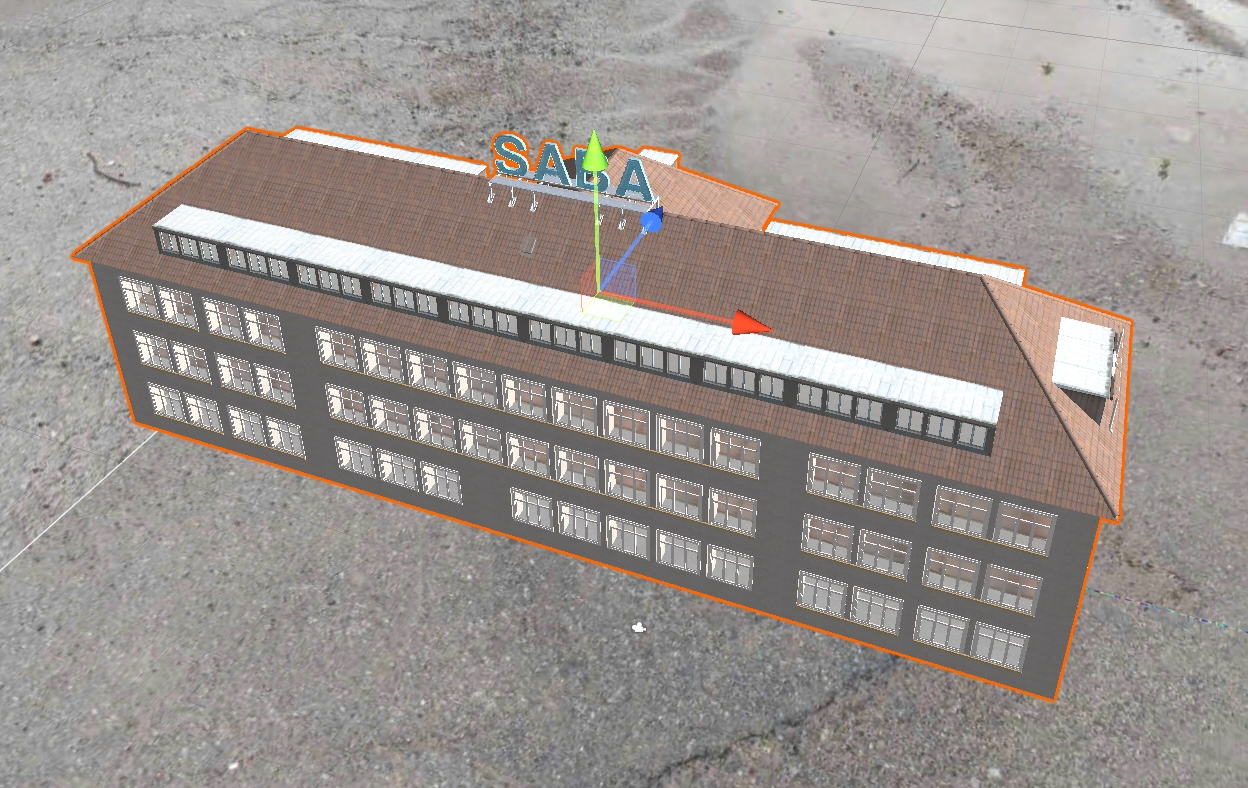
\includegraphics[width=0.5\linewidth]{img/anwendung/technisch/gps/konzeption-lokales-koordinatensystem-saba.jpg}}%
    \qquad
    \subfloat[][]{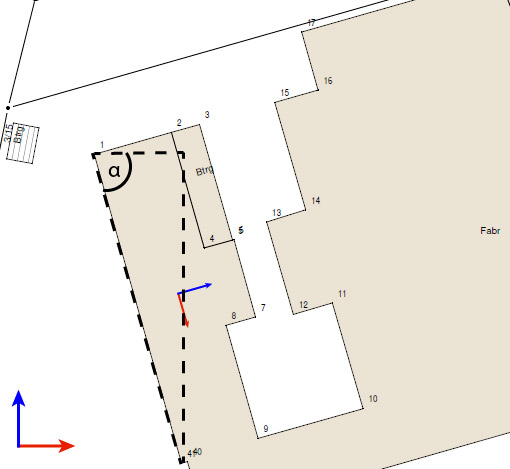
\includegraphics[width=0.4\linewidth]{img/anwendung/technisch/gps/SABA-winkel.jpg}}%
    \caption{Das lokale Koordinatensystem des SABA Gebäudes zeigt mit der z-Richtung (blauer Pfeil) nach Norden(a). Um den Winkel \textalpha  wird das Gebäude gedreht, damit die Rotation des Gebäudes mit den realen Gebäude übereinstimmt(b).}%
    \label{fig:umsetzung-gps-rotation-saba}
\end{figure}

Folgende Winkel werden für die Gebäude in dieser Anwendung verwendet:

\begin{table}[H]
    \centering
    \begin{tabular}{|p{0.25\textwidth}|p{0.04\textwidth}|p{0.4\textwidth}|p{0.15\textwidth}|}
    \hline
        Gebäude                 & Nr. &       lokales Koordinatensystem       & Winkel     \\ \hline 
        SABA                    & 1   & \parbox[c]{0.4\textwidth}{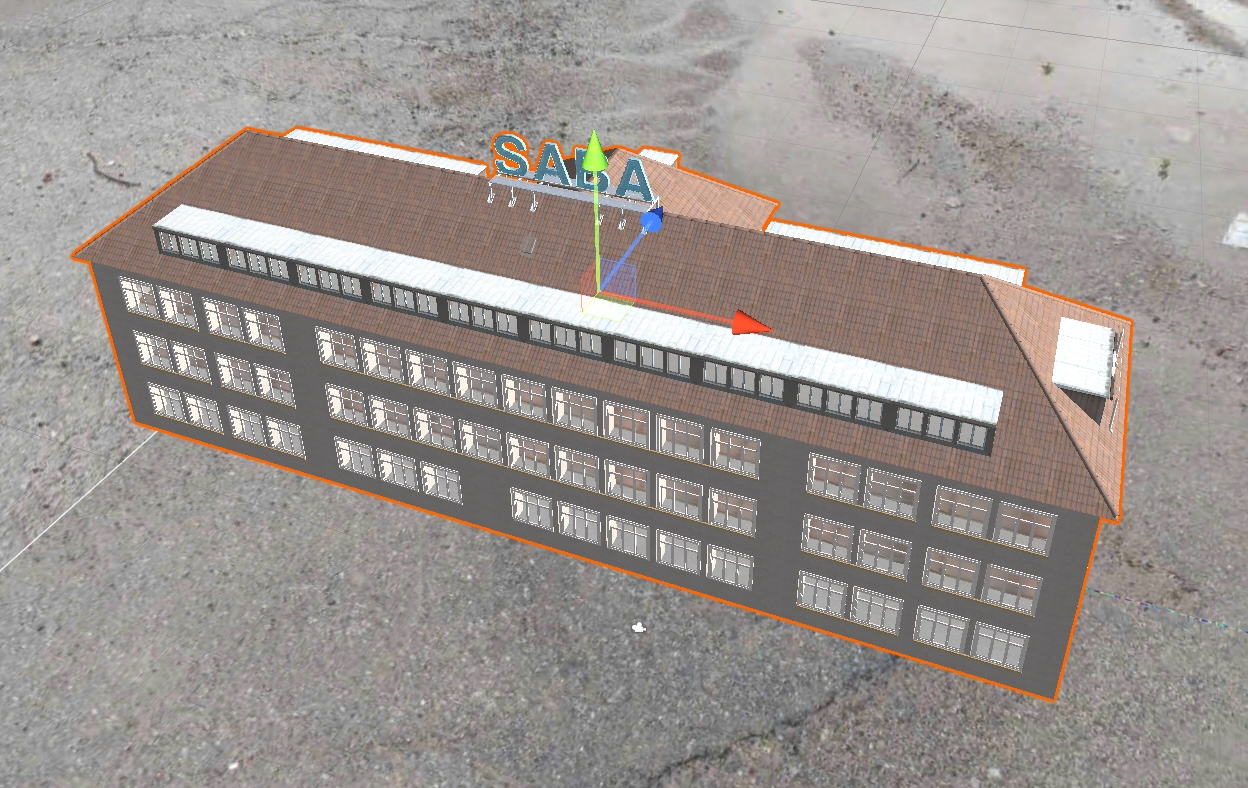
\includegraphics[width=0.4\textwidth]{img/anwendung/technisch/gps/konzeption-lokales-koordinatensystem-saba.jpg}} & 74,32°     \\ \hline
        Reithalle               & 2   & \parbox[c]{0.4\textwidth}{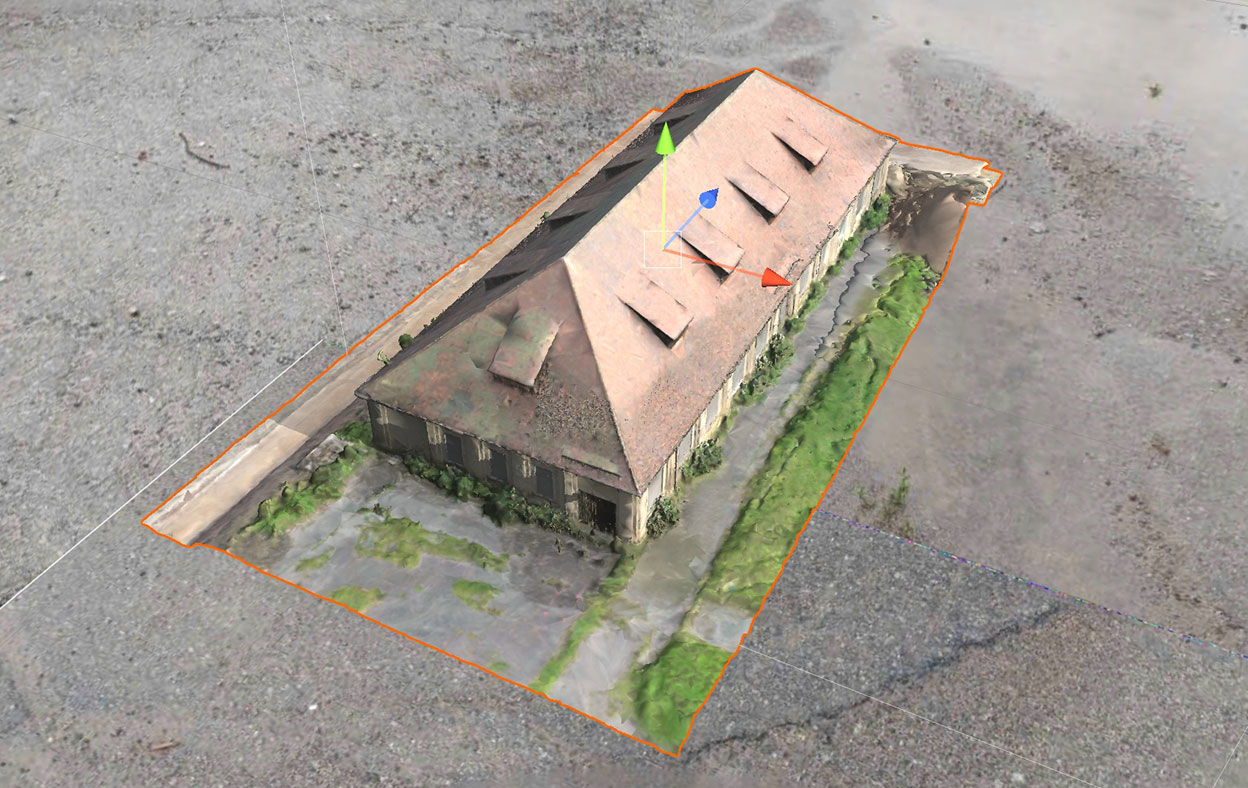
\includegraphics[width=0.4\textwidth]{img/anwendung/technisch/gps/konzeption-lokales-koordinatensystem-l1.jpg}}                                     & 33,54°  \\ \hline
        Mannschaftsgebäude 1    & 3   & \parbox[c]{0.4\textwidth}{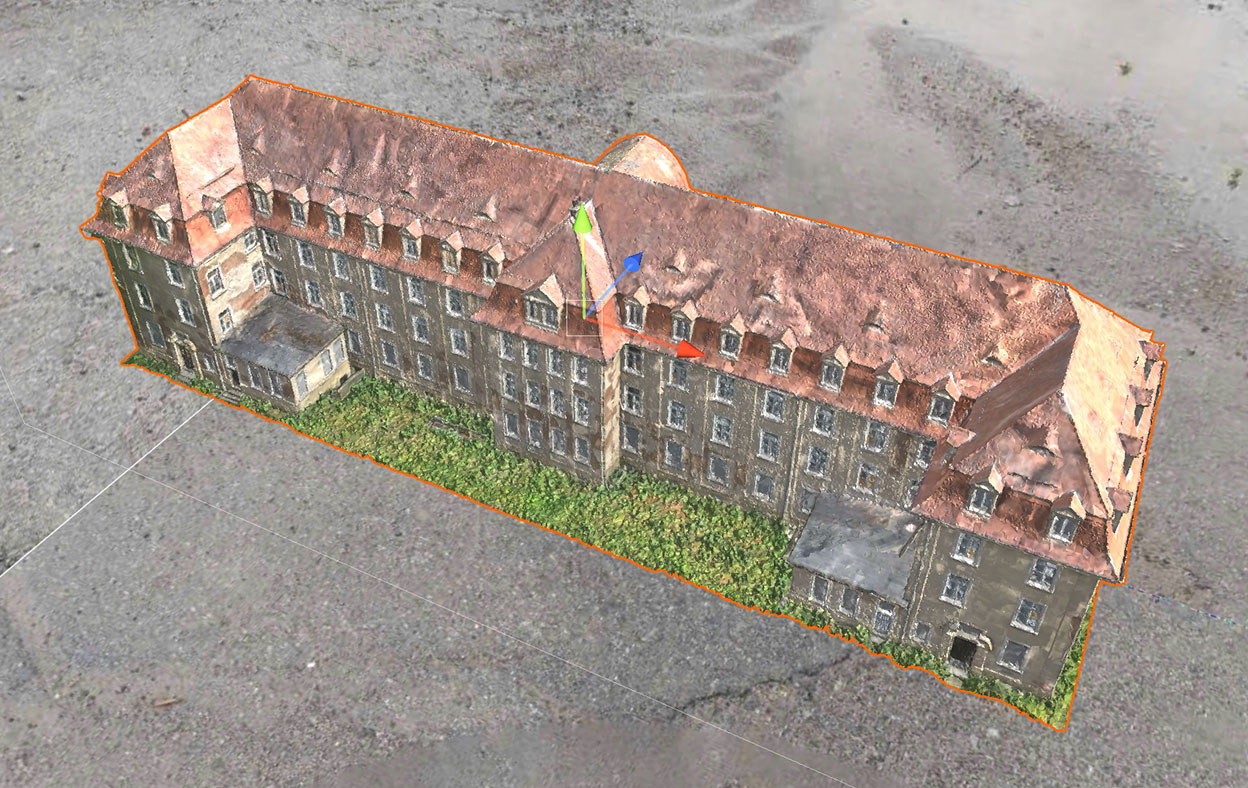
\includegraphics[width=0.4\textwidth]{img/anwendung/technisch/gps/konzeption-lokales-koordinatensystem-l2.jpg}}                                     & 208,00°     \\ \hline
        Wirtschaftsgebäude\footnotemark      & 4   & \parbox[c]{0.4\textwidth}{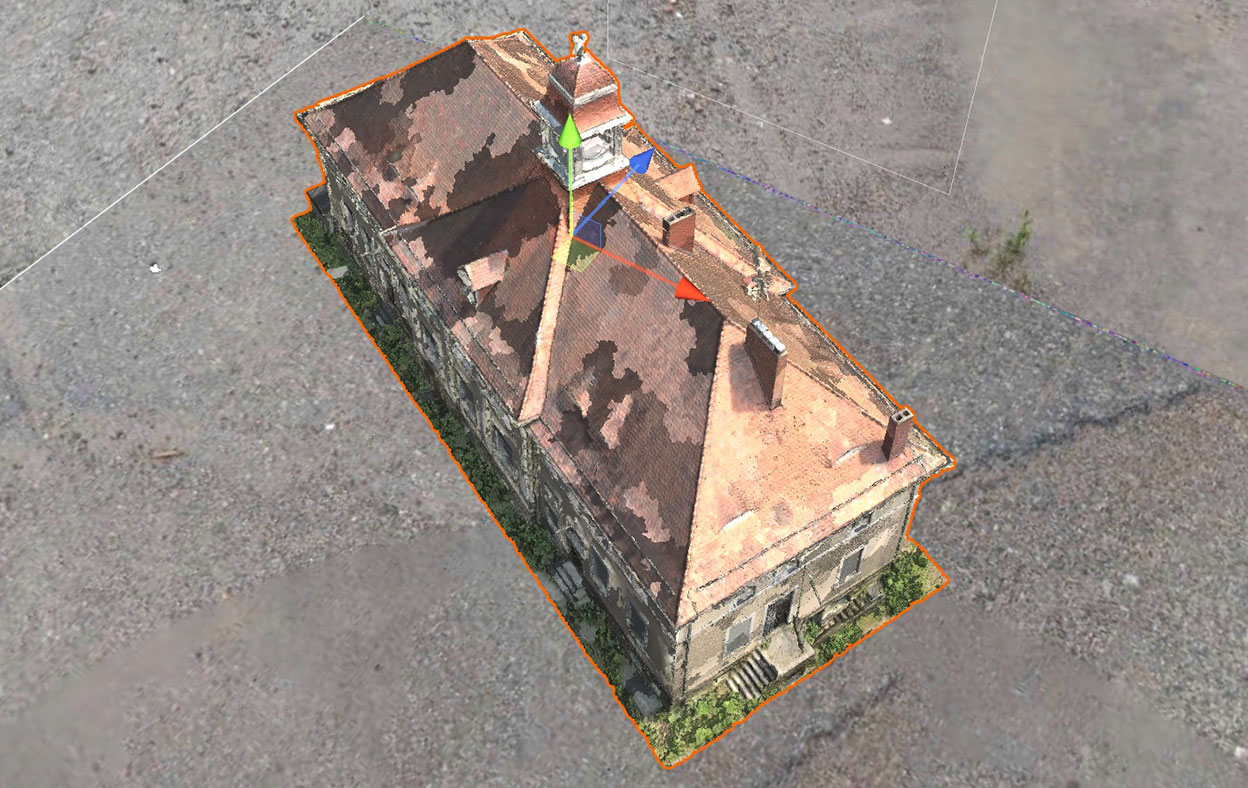
\includegraphics[width=0.4\textwidth]{img/anwendung/technisch/gps/konzeption-lokales-koordinatensystem-l3.jpg}}                                     & 23,10°     \\ \hline
        Mannschaftsgebäude 2    & 5   & \parbox[c]{0.4\textwidth}{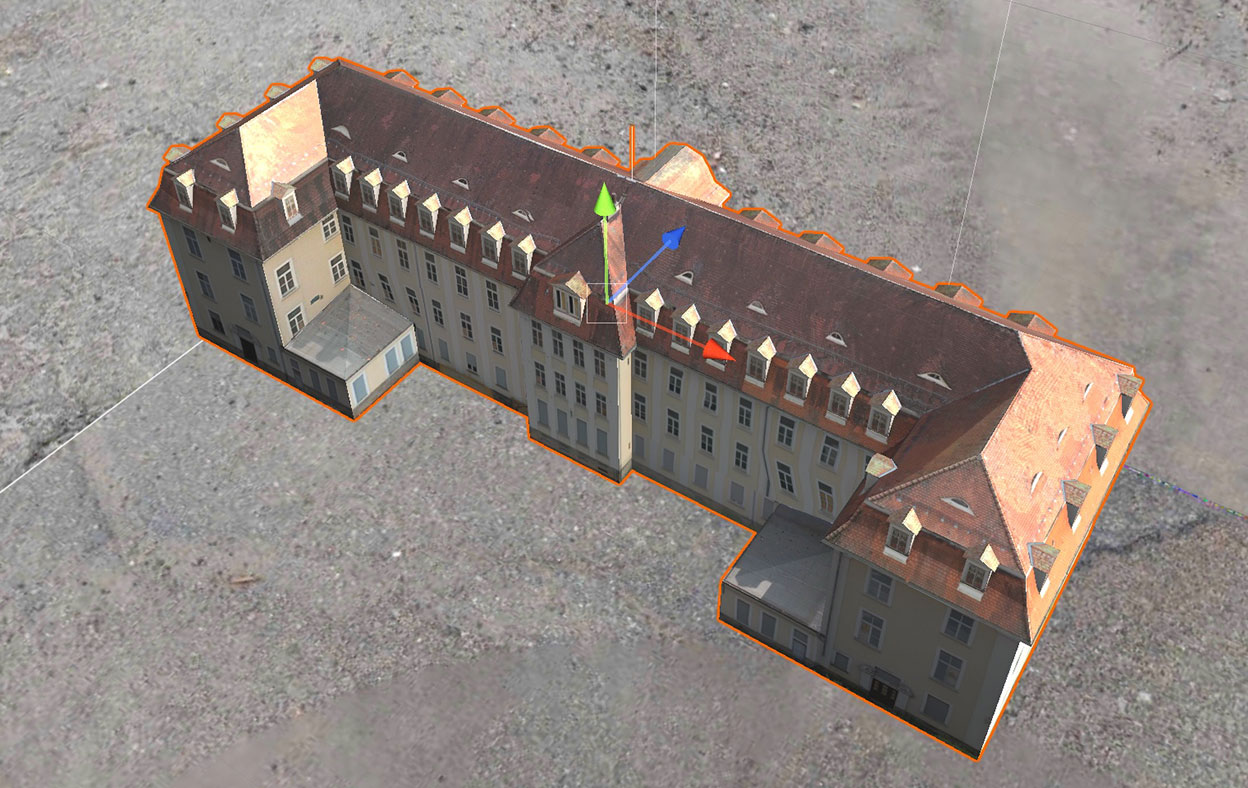
\includegraphics[width=0.4\textwidth]{img/anwendung/technisch/gps/konzeption-lokales-koordinatensystem-l4.jpg}}                                      & 20,40°       \\ \hline
    \end{tabular}
    \caption{Die lokalen Koordinatensysteme der Gebäude und deren Winkelangaben zur korrekten Rotation.}
    \label{tab:umsetzung-gps-berechnete-winkel}
\end{table}

\footnotetext{Wie am Bild in der Tabelle zu sehen, ist das Gebäude bereits um den Winkel rotiert.}

\subsection{Belichtung}
\label{technische-umsetzung-licht}
% Wie wird die Beleuchtung geregelt?
Die Belichtung der Szenen besteht aus drei Komponenten. Mit der Light Estimation API wird der \textit{Ambient Intensity Mode} genutzt, um die durchschnittliche Helligkeit und die durchschnittliche Farbetmperatur zu bestimmen. Mit diesen Werten wird das Hauptlicht gefärbt, um die realen Lichtbedingungen einwirken zu lassen. Das Hauptlicht ist ein direktionales Licht, das die gesamte virtuelle Szene aufhellt. Dieses Licht simuliert die Sonne. Letzlich werden HDR Panoramabilder des SABA Geländes angefertigt, um Cubemaps zu generieren und \textit{Environmental Lighting} zu ermöglichen. In den folgenden Abschnitten wird die Implementierung der verwendeten Techniken gezeigt. Vorher und Nachher Vergleiche zeigen die Unterschiede bei der Belichtung.

\subsubsection{Light Estimation in dieser Anwendung}
\label{technische-umsetzung-light-estimation}



\subsubsection{Sonne simulieren}
% Sonne Setup

\subsection{Wetterbedingungen}
\label{technische-umsetzung-wetterbedingungen}
Dieses Kapitel behandelt die Umsetzung der Veränderungen an der Szene anhand von Wetterdaten. Zunächst wird die auf die Anbindung an die Wetter REST-API in Unity eingegangen. Danach wird veranschaulicht, welche Parameter angepasst werden. Ein anschließender Vergleich der einzelnen Wetterbedingungen zeigt die Auswirkungen auf die Optik der Gebäude. 

\subsubsection{Anbindung der REST-API}
Um Wetterdaten in \textit{Open Weather Map} abzufragen, wird ein Account benötigt. Genutzt wird die \textit{Current Weather} API\footnote{https://openweathermap.org/current, zuletzt aufgerufen am 19.08.2022}. Nach der Anmeldung wird im Account ein API Key generiert, der später im Skript für die Anfrage benötigt wird. 

Die Antwort der API erfolgt über eine \acrfull{json} Datei. Es ist ein Datenformat, das zum Datenaustausch zwischen Anwendungen genutzt wird. JSON Daten liegen in einfach lesbare Textform bereit und ist Programmiersprachen unabhängig\footnote{https://de.wikipedia.org/wiki/JavaScript\_Object\_Notation, zuletzt aufgerufen am 19.08.2022}. Um die Daten der JSON Datei zu nutzen, wird ein JSON-Parser in Unity benötigt. In dieser Anwendung wird SimpleJSON\footnote{https://github.com/Bunny83/SimpleJSON, zuletzt aufgerufen am 19.08.2022} genutzt. Das Skript wird als Asset in das Unity Projekt eingefügt.

Das Wetter wird in der Szene vom \textit{Weather Manager} und dem \texttt{WeatherManager.cs} Skript geregelt. Zunächst wird in einer \textit{Coroutine} durchgeführt, um die Längen- und Breitengrade der aktuellen Position zu ermitteln. Mit einer \textit{Coroutine} werden in Unity Arbeitsschritte durchgeführt. Zum Beispiel wird für eine Funktion 1 das Ergebnis einer anderen Funktion 2 benötigt. Mit einer \textit{Coroutine} wird dafür gesorgt, dass die Funktion 2 ausgeführt wird und Funktion 1 erst dann ausgeführt wird, wenn Funktion 2 vollständig durchlaufen ist. In diesem Fall wird für die Anfrage der Daten die Längen- und Breitengrade benötigt. Erst wenn diese vorhanden sind, erfolgt eine Anfrage der Daten.



\begin{lstlisting}[language=C,caption={Die \texttt{ARPlaceObject()} Funktion.},captionpos=b,label=lst:arplaceobject-funktion]
private IEnumerator FetchWeatherDataFromApi(string latitude, string longitude)
    {
        string url = currentWeatherApi + "lat=" + latitude + "&lon=" + longitude + "&appid=" + apiKey + "&units=metric";
        UnityWebRequest fetchWeatherRequest = UnityWebRequest.Get(url);
        yield return fetchWeatherRequest.SendWebRequest();
        if (fetchWeatherRequest.isNetworkError || fetchWeatherRequest.isHttpError)
        {
            //Check and print error
            statusText.text = fetchWeatherRequest.error;
        }
        else
        {
            Debug.Log(fetchWeatherRequest.downloadHandler.text);
            var response = JSON.Parse(fetchWeatherRequest.downloadHandler.text);

            //set UI Text
            location.text = "Ort: " + response["name"];
            weatherIDText.text = "WetterID: " + response["weather"][0]["id"];
            mainWeather.text = "Wetter: " + response["weather"][0]["main"];
            description.text = "Beschriebung: " + response["weather"][0]["description"];
            temp.text = response["main"]["temp"] + " C";

            //fetch data for further functions
            weatherID = response["weather"][0]["id"];

            if (IsWeatherImpactEnabled.isOn)
            {
                ChooseWeatherCase(weatherID);
            }
        }
    }
\end{lstlisting}
    


\subsubsection{Veränderungen der Wetter Parameter}
% Welche Parameter gibt es?

\subsection{Verwendete Shader}